%%%%%%%%%%%%%%%%%%%%%%%%%%%%%%%%%%%%%%%%%
% The Legrand Orange Book
% LaTeX Template
% Version 2.1 (14/11/15)
%
% This template has been downloaded from:
% http://www.LaTeXTemplates.com
%
% Mathias Legrand (legrand.mathias@gmail.com) with modifications by:
% Vel (vel@latextemplates.com)
%
% License:
% CC BY-NC-SA 3.0 (http://creativecommons.org/licenses/by-nc-sa/3.0/)
%by a multiplication 
% Compiling this template:
% This template uses biber for its bibliography and makeindex for its index.
% When you first open the template, compile it from the command line with the 
% commands below to make sure your LaTeX distribution is configured correctly:
%
% 1) pdflatex main
% 2) makeindex main.idx -s StyleInd.ist
% 3) biber main
% 4) pdflatex main x 2
%
% After this, when you wish to update the bibliography/index use the appropriate
% command above and make sure to compile with pdflatex several times 
% afterwards to propagate your changes to the document.
%
% This template also uses a number of packages which may need to be
% updated to the newest versions for the template to compile. It is strongly
% recommended you update your LaTeX distribution if you have any
% compilation errors.
%
% Important note:
% Chapter heading images should have a 2:1 width:height ratio,
% e.g. 920px width and 460px height.
%
%%%%%%%%%%%%%%%%%%%%%%%%%%%%%%%%%%%%%%%%%

%----------------------------------------------------------------------------------------
%	PACKAGES AND OTHER DOCUMENT CONFIGURATIONS
%----------------------------------------------------------------------------------------

\documentclass[11pt,fleqn]{book} % Default font size and left-justified equations
\usepackage{xcolor,colortbl}
\usepackage{multirow}
\usepackage[export]{adjustbox}
% \newcommand{\TBC} {\vspace {1em} \noindent [TO BE COMPLETED IN THE FINAL VERSION.] \vspace {1em}}
\newcommand{\TBC} {\noindent [TO BE COMPLETED IN THE FINAL VERSION.] }

%----------------------------------------------------------------------------------------

%%%%%%%%%%%%%%%%%%%%%%%%%%%%%%%%%%%%%%%%%
% The Legrand Orange Book
% Structural Definitions File
% Version 2.0 (9/2/15)
%
% Original author:
% Mathias Legrand (legrand.mathias@gmail.com) with modifications by:
% Vel (vel@latextemplates.com)
% 
% This file has been downloaded from:
% http://www.LaTeXTemplates.com
%
% License:
% CC BY-NC-SA 3.0 (http://creativecommons.org/licenses/by-nc-sa/3.0/)
%
%%%%%%%%%%%%%%%%%%%%%%%%%%%%%%%%%%%%%%%%%

%----------------------------------------------------------------------------------------
%	VARIOUS REQUIRED PACKAGES AND CONFIGURATIONS
%----------------------------------------------------------------------------------------

\usepackage[top=3cm,bottom=3cm,left=3cm,right=3cm,headsep=10pt,a4paper]{geometry} % Page margins

\usepackage{upgreek} 
\usepackage{graphicx} % Required for including pictures
\graphicspath{{Pictures/}} % Specifies the directory where pictures are stored

\usepackage{lipsum} % Inserts dummy text

\usepackage{tikz} % Required for drawing custom shapes

\usepackage[english]{babel} % English language/hyphenation

\usepackage{enumitem} % Customize lists
\setlist{nolistsep} % Reduce spacing between bullet points and numbered lists

\usepackage{booktabs} % Required for nicer horizontal rules in tables

\usepackage{xcolor} % Required for specifying colors by name
% \definecolor{ocre}{RGB}{243,102,25} % Define the orange color used for highlighting throughout the book
\definecolor{ocre}{RGB}{203,142,95} % Define the orange color used for highlighting throughout the book

%----------------------------------------------------------------------------------------
%	FONTS
%----------------------------------------------------------------------------------------

\usepackage{avant} % Use the Avantgarde font for headings
%\usepackage{times} % Use the Times font for headings
\usepackage{mathptmx} % Use the Adobe Times Roman as the default text font together with math symbols from the Sym­bol, Chancery and Com­puter Modern fonts

\usepackage{microtype} % Slightly tweak font spacing for aesthetics
\usepackage[utf8]{inputenc} % Required for including letters with accents
\usepackage[T1]{fontenc} % Use 8-bit encoding that has 256 glyphs

%----------------------------------------------------------------------------------------
%	BIBLIOGRAPHY AND INDEX
%----------------------------------------------------------------------------------------
% \usepackage[style=alphabetic,citestyle=numeric,sorting=nyt,sortcites=true,autopunct=true,babel=hyphen,hyperref=true,abbreviate=false,backref=true,backend=biber]{biblatex}
% \addbibresource{bibliography.bib} % BibTeX bibliography file
% \defbibheading{bibempty}{}
% \usepackage[pdftex]{hyperref}


\usepackage{calc} % For simpler calculation - used for spacing the index letter headings correctly
\usepackage{makeidx} % Required to make an index
\makeindex % Tells LaTeX to create the files required for indexing

%----------------------------------------------------------------------------------------
%	MAIN TABLE OF CONTENTS
%----------------------------------------------------------------------------------------

\usepackage{titletoc} % Required for manipulating the table of contents

\contentsmargin{0cm} % Removes the default margin

% Part text styling
\titlecontents{part}[0cm]
{\addvspace{20pt}\centering\large\bfseries}
{}
{}
{}

% Chapter text styling
\titlecontents{chapter}[1.25cm] % Indentation
{\addvspace{12pt}\large\sffamily\bfseries} % Spacing and font options for chapters
{\color{ocre!60}\contentslabel[\Large\thecontentslabel]{1.25cm}\color{ocre}} % Chapter number
{\color{ocre}}  
{\color{ocre!60}\normalsize\;\titlerule*[.5pc]{.}\;\thecontentspage} % Page number

% Section text styling
\titlecontents{section}[1.25cm] % Indentation
{\addvspace{3pt}\sffamily\bfseries} % Spacing and font options for sections
{\contentslabel[\thecontentslabel]{1.25cm}} % Section number
{}
{\hfill\color{black}\thecontentspage} % Page number
[]

% Subsection text styling
\titlecontents{subsection}[1.25cm] % Indentation
{\addvspace{1pt}\sffamily\small} % Spacing and font options for subsections
{\contentslabel[\thecontentslabel]{1.25cm}} % Subsection number
{}
{\ \titlerule*[.5pc]{.}\;\thecontentspage} % Page number
[]

% List of figures
\titlecontents{figure}[0em]
{\addvspace{-5pt}\sffamily}
{\thecontentslabel\hspace*{1em}}
{}
{\ \titlerule*[.5pc]{.}\;\thecontentspage}
[]

% List of tables
\titlecontents{table}[0em]
{\addvspace{-5pt}\sffamily}
{\thecontentslabel\hspace*{1em}}
{}
{\ \titlerule*[.5pc]{.}\;\thecontentspage}
[]

%----------------------------------------------------------------------------------------
%	MINI TABLE OF CONTENTS IN PART HEADS
%----------------------------------------------------------------------------------------

% Chapter text styling
\titlecontents{lchapter}[0em] % Indenting
{\addvspace{15pt}\large\sffamily\bfseries} % Spacing and font options for chapters
{\color{ocre}\contentslabel[\Large\thecontentslabel]{1.25cm}\color{ocre}} % Chapter number
{}  
{\color{ocre}\normalsize\sffamily\bfseries\;\titlerule*[.5pc]{.}\;\thecontentspage} % Page number

% Section text styling
\titlecontents{lsection}[0em] % Indenting
{\sffamily\small} % Spacing and font options for sections
{\contentslabel[\thecontentslabel]{1.25cm}} % Section number
{}
{}

% Subsection text styling
\titlecontents{lsubsection}[.5em] % Indentation
{\normalfont\footnotesize\sffamily} % Font settings
{}
{}
{}

%----------------------------------------------------------------------------------------
%	PAGE HEADERS
%----------------------------------------------------------------------------------------

\usepackage{fancyhdr} % Required for header and footer configuration

\pagestyle{fancy}
\renewcommand{\chaptermark}[1]{\markboth{\sffamily\normalsize\bfseries\chaptername\ \thechapter.\ #1}{}} % Chapter text font settings
\renewcommand{\sectionmark}[1]{\markright{\sffamily\normalsize\thesection\hspace{5pt}#1}{}} % Section text font settings
\fancyhf{} \fancyhead[LE,RO]{\sffamily\normalsize\thepage} % Font setting for the page number in the header
\fancyhead[LO]{\rightmark} % Print the nearest section name on the left side of odd pages
\fancyhead[RE]{\leftmark} % Print the current chapter name on the right side of even pages
\renewcommand{\headrulewidth}{0.5pt} % Width of the rule under the header
\addtolength{\headheight}{2.5pt} % Increase the spacing around the header slightly
\renewcommand{\footrulewidth}{0pt} % Removes the rule in the footer
\fancypagestyle{plain}{\fancyhead{}\renewcommand{\headrulewidth}{0pt}} % Style for when a plain pagestyle is specified

% Removes the header from odd empty pages at the end of chapters
\makeatletter
\renewcommand{\cleardoublepage}{
\clearpage\ifodd\c@page\else
\hbox{}
\vspace*{\fill}
\thispagestyle{empty}
\newpage
\fi}

%----------------------------------------------------------------------------------------
%	THEOREM STYLES
%----------------------------------------------------------------------------------------

\usepackage{amsmath,amsfonts,amssymb,amsthm} % For math equations, theorems, symbols, etc

\newcommand{\intoo}[2]{\mathopen{]}#1\,;#2\mathclose{[}}
\newcommand{\ud}{\mathop{\mathrm{{}d}}\mathopen{}}
\newcommand{\intff}[2]{\mathopen{[}#1\,;#2\mathclose{]}}
\newtheorem{notation}{Notation}[chapter]

% Boxed/framed environments
\newtheoremstyle{ocrenumbox}% % Theorem style name
{0pt}% Space above
{0pt}% Space below
{\normalfont}% % Body font
{}% Indent amount
{\small\bf\sffamily\color{ocre}}% % Theorem head font
{\;}% Punctuation after theorem head
{0.25em}% Space after theorem head
{\small\sffamily\color{ocre}\thmname{#1}\nobreakspace\thmnumber{\@ifnotempty{#1}{}\@upn{#2}}% Theorem text (e.g. Theorem 2.1)
\thmnote{\nobreakspace\the\thm@notefont\sffamily\bfseries\color{black}---\nobreakspace#3.}} % Optional theorem note
\renewcommand{\qedsymbol}{$\blacksquare$}% Optional qed square

\newtheoremstyle{blacknumex}% Theorem style name
{5pt}% Space above
{5pt}% Space below
{\normalfont}% Body font
{} % Indent amount
{\small\bf\sffamily}% Theorem head font
{\;}% Punctuation after theorem head
{0.25em}% Space after theorem head
{\small\sffamily{\tiny\ensuremath{\blacksquare}}\nobreakspace\thmname{#1}\nobreakspace\thmnumber{\@ifnotempty{#1}{}\@upn{#2}}% Theorem text (e.g. Theorem 2.1)
\thmnote{\nobreakspace\the\thm@notefont\sffamily\bfseries---\nobreakspace#3.}}% Optional theorem note

\newtheoremstyle{blacknumbox} % Theorem style name
{0pt}% Space above
{0pt}% Space below
{\normalfont}% Body font
{}% Indent amount
{\small\bf\sffamily}% Theorem head font
{\;}% Punctuation after theorem head
{0.25em}% Space after theorem head
{\small\sffamily\thmname{#1}\nobreakspace\thmnumber{\@ifnotempty{#1}{}\@upn{#2}}% Theorem text (e.g. Theorem 2.1)
\thmnote{\nobreakspace\the\thm@notefont\sffamily\bfseries---\nobreakspace#3.}}% Optional theorem note

% Non-boxed/non-framed environments
\newtheoremstyle{ocrenum}% % Theorem style name
{5pt}% Space above
{5pt}% Space below
{\normalfont}% % Body font
{}% Indent amount
{\small\bf\sffamily\color{ocre}}% % Theorem head font
{\;}% Punctuation after theorem head
{0.25em}% Space after theorem head
{\small\sffamily\color{ocre}\thmname{#1}\nobreakspace\thmnumber{\@ifnotempty{#1}{}\@upn{#2}}% Theorem text (e.g. Theorem 2.1)
\thmnote{\nobreakspace\the\thm@notefont\sffamily\bfseries\color{black}---\nobreakspace#3.}} % Optional theorem note
\renewcommand{\qedsymbol}{$\blacksquare$}% Optional qed square
\makeatother

% Defines the theorem text style for each type of theorem to one of the three styles above
\newcounter{dummy} 
\numberwithin{dummy}{section}
\theoremstyle{ocrenumbox}
\newtheorem{theoremeT}[dummy]{Theorem}
\newtheorem{problem}{Problem}[chapter]
\newtheorem{exerciseT}{Exercise}[chapter]
\theoremstyle{blacknumex}
\newtheorem{exampleT}{Example}[chapter]
\theoremstyle{blacknumbox}
\newtheorem{vocabulary}{Vocabulary}[chapter]
\newtheorem{definitionT}{Definition}[section]
\newtheorem{corollaryT}[dummy]{Corollary}
\theoremstyle{ocrenum}
\newtheorem{proposition}[dummy]{Proposition}

%----------------------------------------------------------------------------------------
%	DEFINITION OF COLORED BOXES
%----------------------------------------------------------------------------------------

\RequirePackage[framemethod=default]{mdframed} % Required for creating the theorem, definition, exercise and corollary boxes

% Theorem box
\newmdenv[skipabove=7pt,
skipbelow=7pt,
backgroundcolor=black!5,
linecolor=ocre,
innerleftmargin=5pt,
innerrightmargin=5pt,
innertopmargin=5pt,
leftmargin=0cm,
rightmargin=0cm,
innerbottommargin=5pt]{tBox}

% Exercise box	  
\newmdenv[skipabove=7pt,
skipbelow=7pt,
rightline=false,
leftline=true,
topline=false,
bottomline=false,
backgroundcolor=ocre!10,
linecolor=ocre,
innerleftmargin=5pt,
innerrightmargin=5pt,
innertopmargin=5pt,
innerbottommargin=5pt,
leftmargin=0cm,
rightmargin=0cm,
linewidth=4pt]{eBox}	

% Definition box
\newmdenv[skipabove=7pt,
skipbelow=7pt,
rightline=false,
leftline=true,
topline=false,
bottomline=false,
linecolor=ocre,
innerleftmargin=5pt,
innerrightmargin=5pt,
innertopmargin=0pt,
leftmargin=0cm,
rightmargin=0cm,
linewidth=4pt,
innerbottommargin=0pt]{dBox}	

% Corollary box
\newmdenv[skipabove=7pt,
skipbelow=7pt,
rightline=false,
leftline=true,
topline=false,
bottomline=false,
linecolor=gray,
backgroundcolor=black!5,
innerleftmargin=5pt,
innerrightmargin=5pt,
innertopmargin=5pt,
leftmargin=0cm,
rightmargin=0cm,
linewidth=4pt,
innerbottommargin=5pt]{cBox}

% Creates an environment for each type of theorem and assigns it a theorem text style from the "Theorem Styles" section above and a colored box from above
\newenvironment{theorem}{\begin{tBox}\begin{theoremeT}}{\end{theoremeT}\end{tBox}}
\newenvironment{exercise}{\begin{eBox}\begin{exerciseT}}{\hfill{\color{ocre}\tiny\ensuremath{\blacksquare}}\end{exerciseT}\end{eBox}}				  
\newenvironment{definition}{\begin{dBox}\begin{definitionT}}{\end{definitionT}\end{dBox}}	
\newenvironment{example}{\begin{exampleT}}{\hfill{\tiny\ensuremath{\blacksquare}}\end{exampleT}}		
\newenvironment{corollary}{\begin{cBox}\begin{corollaryT}}{\end{corollaryT}\end{cBox}}	

%----------------------------------------------------------------------------------------
%	REMARK ENVIRONMENT
%----------------------------------------------------------------------------------------

\newenvironment{remark}{\par\vspace{10pt}\small % Vertical white space above the remark and smaller font size
\begin{list}{}{
\leftmargin=35pt % Indentation on the left
\rightmargin=25pt}\item\ignorespaces % Indentation on the right
\makebox[-2.5pt]{\begin{tikzpicture}[overlay]
\node[draw=ocre!60,line width=1pt,circle,fill=ocre!25,font=\sffamily\bfseries,inner sep=2pt,outer sep=0pt] at (-15pt,0pt){\textcolor{ocre}{R}};\end{tikzpicture}} % Orange R in a circle
\advance\baselineskip -1pt}{\end{list}\vskip5pt} % Tighter line spacing and white space after remark

%----------------------------------------------------------------------------------------
%	SECTION NUMBERING IN THE MARGIN
%----------------------------------------------------------------------------------------

\makeatletter
\renewcommand{\@seccntformat}[1]{\llap{\textcolor{ocre}{\csname the#1\endcsname}\hspace{1em}}}                    
\renewcommand{\section}{\@startsection{section}{1}{\z@}
{-4ex \@plus -1ex \@minus -.4ex}
{1ex \@plus.2ex }
{\normalfont\large\sffamily\bfseries}}
\renewcommand{\subsection}{\@startsection {subsection}{2}{\z@}
{-3ex \@plus -0.1ex \@minus -.4ex}
{0.5ex \@plus.2ex }
{\normalfont\sffamily\bfseries}}
\renewcommand{\subsubsection}{\@startsection {subsubsection}{3}{\z@}
{-2ex \@plus -0.1ex \@minus -.2ex}
{.2ex \@plus.2ex }
{\normalfont\small\sffamily\bfseries}}                        
\renewcommand\paragraph{\@startsection{paragraph}{4}{\z@}
{-2ex \@plus-.2ex \@minus .2ex}
{.1ex}
{\normalfont\small\sffamily\bfseries}}

%----------------------------------------------------------------------------------------
%	PART HEADINGS
%----------------------------------------------------------------------------------------

% numbered part in the table of contents
\newcommand{\@mypartnumtocformat}[2]{%
\setlength\fboxsep{0pt}%
\noindent\colorbox{ocre!20}{\strut\parbox[c][.7cm]{\ecart}{\color{ocre!70}\Large\sffamily\bfseries\centering#1}}\hskip\esp\colorbox{ocre!40}{\strut\parbox[c][.7cm]{\linewidth-\ecart-\esp}{\Large\sffamily\centering#2}}}%
%%%%%%%%%%%%%%%%%%%%%%%%%%%%%%%%%%
% unnumbered part in the table of contents
\newcommand{\@myparttocformat}[1]{%
\setlength\fboxsep{0pt}%
\noindent\colorbox{ocre!40}{\strut\parbox[c][.7cm]{\linewidth}{\Large\sffamily\centering#1}}}%
%%%%%%%%%%%%%%%%%%%%%%%%%%%%%%%%%%
\newlength\esp
\setlength\esp{4pt}
\newlength\ecart
\setlength\ecart{1.2cm-\esp}
\newcommand{\thepartimage}{}%
\newcommand{\partimage}[1]{\renewcommand{\thepartimage}{#1}}%
\def\@part[#1]#2{%
\ifnum \c@secnumdepth >-2\relax%
\refstepcounter{part}%
\addcontentsline{toc}{part}{\texorpdfstring{\protect\@mypartnumtocformat{\thepart}{#1}}{\partname~\thepart\ ---\ #1}}
\else%
\addcontentsline{toc}{part}{\texorpdfstring{\protect\@myparttocformat{#1}}{#1}}%
\fi%
\startcontents%
\markboth{}{}%
{\thispagestyle{empty}%
\begin{tikzpicture}[remember picture,overlay]%
\node at (current page.north west){\begin{tikzpicture}[remember picture,overlay]%	
\fill[ocre!20](0cm,0cm) rectangle (\paperwidth,-\paperheight);
\node[anchor=north] at (4cm,-3.25cm){\color{ocre!40}\fontsize{220}{100}\sffamily\bfseries\@Roman\c@part}; 
\node[anchor=south east] at (\paperwidth-1cm,-\paperheight+1cm){\parbox[t][][t]{8.5cm}{
\printcontents{l}{0}{\setcounter{tocdepth}{1}}%
}};
\node[anchor=north east] at (\paperwidth-1.5cm,-3.25cm){\parbox[t][][t]{15cm}{\strut\raggedleft\color{white}\fontsize{30}{30}\sffamily\bfseries#2}};
\end{tikzpicture}};
\end{tikzpicture}}%
\@endpart}
\def\@spart#1{%
\startcontents%
\phantomsection
{\thispagestyle{empty}%
\begin{tikzpicture}[remember picture,overlay]%
\node at (current page.north west){\begin{tikzpicture}[remember picture,overlay]%	
\fill[ocre!20](0cm,0cm) rectangle (\paperwidth,-\paperheight);
\node[anchor=north east] at (\paperwidth-1.5cm,-3.25cm){\parbox[t][][t]{15cm}{\strut\raggedleft\color{white}\fontsize{30}{30}\sffamily\bfseries#1}};
\end{tikzpicture}};
\end{tikzpicture}}
\addcontentsline{toc}{part}{\texorpdfstring{%
\setlength\fboxsep{0pt}%
\noindent\protect\colorbox{ocre!40}{\strut\protect\parbox[c][.7cm]{\linewidth}{\Large\sffamily\protect\centering #1\quad\mbox{}}}}{#1}}%
\@endpart}
\def\@endpart{\vfil\newpage
\if@twoside
\if@openright
\null
\thispagestyle{empty}%
\newpage
\fi
\fi
\if@tempswa
\twocolumn
\fi}

%----------------------------------------------------------------------------------------
%	CHAPTER HEADINGS
%----------------------------------------------------------------------------------------

\newcommand{\thechapterimage}{}%
\newcommand{\chapterimage}[1]{\renewcommand{\thechapterimage}{#1}}%
\def\@makechapterhead#1{%
{\parindent \z@ \raggedright \normalfont
\ifnum \c@secnumdepth >\m@ne
\if@mainmatter
\begin{tikzpicture}[remember picture,overlay]
\node at (current page.north west)
{\begin{tikzpicture}[remember picture,overlay]
\node[anchor=north west,inner sep=0pt] at (0,0) {\includegraphics[width=\paperwidth]{\thechapterimage}};
% \draw[anchor=west] (\Gm@lmargin,-9cm) node [line width=2pt,rounded corners=15pt,draw=ocre,fill=white,fill opacity=0.5,inner sep=15pt]{\strut\makebox[22cm]{}};
\draw[anchor=west] (\Gm@lmargin+.3cm,-3cm) node {\huge\sffamily\bfseries\color{black}\thechapter. #1\strut};
% \draw[anchor=west] (\Gm@lmargin+.3cm,-9cm) node {\huge\sffamily\bfseries\color{black}\thechapter. #1\strut};
\end{tikzpicture}};
\end{tikzpicture}
\else
\begin{tikzpicture}[remember picture,overlay]
\node at (current page.north west)
{\begin{tikzpicture}[remember picture,overlay]
\node[anchor=north west,inner sep=0pt] at (0,0) {\includegraphics[width=\paperwidth]{\thechapterimage}};
\draw[anchor=west] (\Gm@lmargin,-9cm) node [line width=2pt,rounded corners=15pt,draw=ocre,fill=white,fill opacity=0.5,inner sep=15pt]{\strut\makebox[22cm]{}};
\draw[anchor=west] (\Gm@lmargin+.3cm,-9cm) node {\huge\sffamily\bfseries\color{black}#1\strut};
\end{tikzpicture}};
\end{tikzpicture}
% \fi\fi\par\vspace*{270\p@}}}
\fi\fi\par\vspace*{70\p@}}}

%-------------------------------------------

\def\@makeschapterhead#1{%
\begin{tikzpicture}[remember picture,overlay]
\node at (current page.north west)
{\begin{tikzpicture}[remember picture,overlay]
\node[anchor=north west,inner sep=0pt] at (0,0) {\includegraphics[width=\paperwidth]{\thechapterimage}};
% \draw[anchor=west] (\Gm@lmargin,-9cm) node [line width=1pt,rounded corners=15pt,draw=ocre,fill=white,fill opacity=0.5,inner sep=15pt]{\strut\makebox[22cm]{}};
\draw[anchor=west] (\Gm@lmargin+.3cm,-3cm) node {\huge\sffamily\bfseries\color{black}#1\strut};
\end{tikzpicture}};
\end{tikzpicture}
% \par\vspace*{270\p@}}
\par\vspace*{70\p@}}
\makeatother

%----------------------------------------------------------------------------------------
%	HYPERLINKS IN THE DOCUMENTS
%----------------------------------------------------------------------------------------

\usepackage{hyperref}
\hypersetup{hidelinks,backref=true,pagebackref=true,hyperindex=true,colorlinks=false,breaklinks=true,urlcolor= ocre,bookmarks=true,bookmarksopen=false,pdftitle={Title},pdfauthor={Author}}
\usepackage{bookmark}
\bookmarksetup{
open,
numbered,
addtohook={%
\ifnum\bookmarkget{level}=0 % chapter
\bookmarksetup{bold}%
\fi
\ifnum\bookmarkget{level}=-1 % part
\bookmarksetup{color=ocre,bold}%
\fi
}
} % Insert the commands.tex file which contains the majority of the structure behind the template
%!TEX root = main.tex

%Comments
\newcommand\NeedRef{{\color{red!80}\textbf{Missing ref}}}
\newcommand\NeedFigure{[{\color{red!80}\textbf{Missing figure}}]}
% \newcommand\WJ[1]{[{\color{magenta!80}\textbf{WJ: #1}}]}
\newcommand\WJ[1]{}
\newcommand\CommentGS[1]{[{\color{blue!80}\textbf{GS: #1}}]}
%\newcommand\Todo{{\color{red!80}\textbf{\large TO DO}}}

%References
\newcommand\RefEq[1]{Eq.~(\ref{eq:#1})}
\newcommand\RefEqNum[1]{(\ref{eq:#1})}
\newcommand\RefFig[1]{Fig.~\ref{fig:#1}}
\newcommand\RefFigure[1]{Figure~\ref{fig:#1}}
\newcommand\RefFigNum[1]{\ref{fig:#1}}
\newcommand\RefSubFig[2]{Fig.~\ref{fig:#1}~(#2)}
\newcommand\RefAppendix[1]{Appendix~\ref{sec:#1}}
\newcommand\RefSec[1]{Sec.~\ref{sec:#1}}
\newcommand\RefSecNum[1]{~\ref{sec:#1}}
\newcommand\RefSubSec[1]{Sec.~\ref{subsec:#1}}
\newcommand\RefTable[1]{Table~\ref{tab:#1}}
\newcommand\RefTableNum[1]{\ref{tab:#1}}

%%Math
\newcommand\Dirac{\delta}
\newcommand\Diff{d}
\newcommand\Lebesgue[1]{{\mu(#1)}}
\newcommand{\EqDef}{\!\ensuremath{\mathrel{\mathop:}=}\!}
\newcommand\BigO[1]{\mathcal{O}\!\left(#1\right)}
%\newcommand\Exp[1]{e^{#1}}
\newcommand{\transpose}{^{\top}}
\newcommand{\dif}{\mathrm{d}}
\newcommand\Sinc[1]{\text{Sinc{$\left(#1\right)$}}}
\newcommand\IntegerDomain{\mathbb{N}}
\newcommand\ZeroVector{\mathbb{0}}
\newcommand\InnerProduct[2]{#1\cdot#2 }


%Polar Coordinates
\newcommand\AngularDom{\textbf{n}}

%Cartesian
\newcommand\CanonicalVar[1]{\xi_{#1}}
\newcommand\Vector[1]{
\ifthenelse{\isempty{#1}}
    {\textbf{x}}           % if #1 is empty
    {\textbf{x}_{#1}}    % if #1 is not empty
}


%Matrix
\newcommand\Transpose[1]{{#1}^T}

%Complex numbers
\newcommand\Complex{i}
\newcommand\RealPart[1]{Re\left(#1\right)}
\newcommand\ImagPart[1]{Im\left(#1\right)}
\newcommand\Conjugate[1]{\overline{#1}}
\newcommand\Iota{i}
\newcommand\Norm[1]{||#1||^2}

%Probability and stats
\newcommand\Mean[1]{\left\langle #1 \right\rangle}
\newcommand\VarianceName{\textit{Var}}
\newcommand\CovarianceName{\textit{Cov}}
\newcommand\Variance[1]{\VarianceName\left(#1\right)}
\newcommand\Covariance[2]{\CovarianceName\left(#1,#2\right)}
\newcommand\SampleCovariance[1]{\CovarianceName_{s}\left(#1\right)}
\newcommand\Bias[1]{Bias\left(#1\right)}
\newcommand\MSE[1]{MSE\left(#1\right)}
\newcommand\PDF[1]{g\left(#1\right)}
\newcommand\InvPDF[1]{\alpha \left(#1\right)}
\newcommand\PDFFunc{g}

%FourierTransform
\newcommand\Fourier[1]{\mathcal{F}_{#1}}
\newcommand\FourierRe[1]{\mathcal{R}_{#1}}
\newcommand\FourierIm[1]{\mathcal{I}_{#1}}
\newcommand\FourierAmp[1]{\mathcal{A}_{#1}}
\newcommand\FourierPhase[1]{\Phi_{#1}}
\newcommand\PowerSpec[1]{\mathcal{P}_{#1}}
\newcommand\RadialPowerSpec[1]{\breve{\mathcal{P}_{#1}}}
\newcommand\PowerTerm[2]{\breve{\mathcal{P}_{#1}}\left(#2\right)}
\newcommand\PowerConstant{\gamma}
\newcommand\RadialFreq{\rho}
\newcommand\Power[1]{\mathcal{P}_{#1}}
%\newcommand\Power[1]{\mathcal{P}(#1)}
\newcommand\Frequency[1]{
\ifthenelse{\isempty{#1}}%
    {\omega}% if #1 is empty
    {\omega_{#1}}% if #1 is not empty
}

%DifferentialDomain
\newcommand\PowerDifferential[1]{\mathcal{P}_{#1}^{d}}
%Sampling
\newcommand\Npts{N}

%Domain
\newcommand\Dim[1][D]{{#1}}
\newcommand\SamplingDom{{\mathbb{D}}}
\newcommand\ToroidalDom[1]{{\mathcal{T}^#1}}
\newcommand\FourierDom{{\Theta}}
\newcommand\FourierDomDCPeak{\Phi}
\newcommand\EuclidDom[1]{{\mathbb{R}^{#1}}}
\newcommand\SphericalDom[1]{{\mathcal{S}^{#1}}}
%\newcommand\DifferentialMetric{{d}}

%Spherical Harmonics
\newcommand\SPH[1]{\mathcal{S}_{#1}}
\newcommand\SharmonicAmp[2]{\mathcal{A}_{#1}^{#2}}
\newcommand\SharmonicPhase[2]{\Phi_{#1}^{#2}}
\newcommand\Sconstant[2]{c_{#1}^{#2}}

%Monte Carlo estimation
\newcommand\Integrand{{f}}
\newcommand\Integral{{I}}
\newcommand\RvMCE{{\boldsymbol{I}_\Npts}}
\newcommand\DummyIntegrand{{G}}

%Variables
\newcommand{\sampleSpatial}{\mathbf{s}}
\newcommand{\pointSpatial}{\mathbf{x}}
\newcommand\SpaceVar{\pointSpatial}
\newcommand{\FreqVar}{\mathbf{\omega}}
\newcommand\PolynomialDegree{b}
\newcommand\WorstCase{W}
\newcommand\BestCase{B}
\newcommand\DummyVar{y}
\newcommand\ExtinctionCoeff{\sigma}

\newcommand\cdash[1]{\texttt{-}#1}
\newcommand\cdashs[1]{\texttt{-{}-}#1}

%Sampler
\newcommand\Sampling{S}
\newcommand\RvSampling{\textbf{S}}

% Misc.
\newcommand{\txtblue}[1]{\textcolor{blue}{#1}} 
\newcommand{\txtgreen}[1]{\textcolor{green}{#1}} 
\newcommand{\txtred}[1]{\textcolor{red}{#1}}


\newcommand{\IGNORE} [1] {#1} %% use to remove comments


\newcommand{\KARTIC} [1] {\IGNORE{\textcolor{red} {KARTIC:#1}}}
\newcommand{\GURPRIT} [1] {\IGNORE{\textcolor{blue} {[GURPRIT:#1]}}}
\newcommand{\WOJCIECH} [1] {\IGNORE{\textcolor{brown} {[WOJCIECH:#1]}}}


% % % % % % % New variables (this course)
\newcommand{\pth} {\ensuremath{\bar{p}}}
\newcommand{\xs} {\ensuremath{j}}
\newcommand{\Ij}[1] {\ensuremath{I_{#1}}}


%%%%%%%%%%%%%%%%%%%%%%%%%%%%%%%%%% OLD STUFF 

% % % % % % %  General
\newcommand{\imag}{\ensuremath{\mathrm{\imath}}}
\newcommand{\MyExp}[1] {\ensuremath{\e^{#1}}}
\newcommand{\cn} [2]{\ensuremath{#1+\imag#2}}
\newcommand{\cp} [2]{\ensuremath{#1 \, \MyExp{-\imag #2}}}
\newcommand{\RV}[1] {\ensuremath{\mathbf{#1}}}
\newcommand{\Real}[1] {\ensuremath{\Re(#1)}}
\newcommand{\Imag}[1] {\ensuremath{\Im (#1)}}
\newcommand{\Exp}[1] {\ensuremath{\langle #1 \rangle}}
\newcommand{\Ampl} [1]{\ensuremath{ |#1 |}}
\newcommand{\Phase} [1]{\ensuremath{ \MyExp{\Phi({#1})}}}
% \newcommand{\Ampl} [1]{\ensuremath{\left| #1 \right|}}
% \newcommand{\Exp}[1] {\ensuremath{\left \langle #1 \right \rangle}}
\newcommand{\Var}[1] {\ensuremath{\mathrm{V} \left(#1\right)}}
\newcommand{\Cov}[2] {\ensuremath{\mathrm{Cov} (#1, #2)}}
\newcommand{\e}{\ensuremath{\mathrm{e}}}
\newcommand{\Z}{\ensuremath{\mathbb{Z}}}
\newcommand{\C}{\ensuremath{\mathbb{C}}}
\newcommand{\R}{\ensuremath{\mathbb{R}}}
\newcommand{\conv}{\ensuremath{\otimes}}
\newcommand{\sinc} [1] {\ensuremath{\mathrm{sinc(#1)}}}
\newcommand{\twopartdef}[4]
{
	\left\{
		\begin{array}{ll}
			#1 & \mbox{if } #2 \\
			#3 & \mbox{} #4
		\end{array}
	\right.
}
\newcommand{\DefInt}[4] {\int\limits_{#1}^{#2} \; #3 \;\; \mathrm{d}#4}
\newcommand{\Int}[2] {\int  #1 \; \mathrm{d}#2}
 
% % % % % % % Variables
\newcommand{\N} {\ensuremath{N}}
\newcommand{\rv} {\ensuremath{\varsigma}}
\newcommand{\Est} {\ensuremath{\mathbb{E}}}
\newcommand{\bias} {\ensuremath{\mathcal{B}}}
\newcommand{\var} {\ensuremath{\mathcal{V}}}
\newcommand{\err} {\ensuremath{\Delta}}
\newcommand{\Estim}[1] {\ensuremath{\RV F_{#1}}}

% % % % % % %  Primal
\newcommand{\sfsym} {\ensuremath{\RV S}}
\newcommand{\sdsym} {\ensuremath{g}}
\newcommand{\ifsym} {\ensuremath{f}}
\newcommand{\x} {\ensuremath{x}}
\newcommand{\w} {\ensuremath{\alpha}}
\newcommand{\xii} {\ensuremath{\RV X _i}}
\newcommand{\wii} {\ensuremath{\w_i}}
\newcommand{\Tx} {\ensuremath{T}}
\newcommand{\sfn} {\ensuremath{\sfsym(\x)}}
\newcommand{\sfnp} {\ensuremath{\sfsym'(\x)}}
\newcommand{\ifn} {\ensuremath{\ifsym(\x)}}
\newcommand{\ifnb} {\ensuremath{\ifsym_{\Pi}(\x)}}
\newcommand{\sdn} {\ensuremath{\sdsym(\x)}}
\newcommand{\boxf} [2]{\ensuremath{\Pi_{#1}^{#2}(\x)}}
\newcommand{\shaf} [1]{\ensuremath{{\bot\hspace{-.7ex}\bot\hspace{-.7ex}\bot}_{#1}(\x)}}
 
% % % % % % %  Fourier
\newcommand{\fv} {\ensuremath{\omega}}
\newcommand{\ifv} {\ensuremath{b}}
\newcommand{\rfv} {\ensuremath{a}}
\newcommand{\amp} {\ensuremath{\rho(\omega)}}
\newcommand{\ph} {\ensuremath{\phi(\omega)}}
\newcommand{\FTsym} [1] {\ensuremath{\hat{#1}}}
\newcommand{\FT} [1] {\ensuremath{\hat{#1}(\fv)}}
\newcommand{\SF} {\ensuremath{\FT{\sfsym}}}
\newcommand{\SFp} {\ensuremath{\FTsym{\sfsym}'(\fv)}}
\newcommand{\IFn} {\ensuremath{\FT{\ifsym}}}
\newcommand{\IFnb} {\ensuremath{\FT{\ifsym_{\Pi}}}}
\newcommand{\SFsym} {\ensuremath{\FTsym{\sfsym}}}
\newcommand{\IFsym} {\ensuremath{\FTsym{\ifsym}}}
\newcommand{\BOXF} [2]{\ensuremath{\FTsym{\Pi}_{#1}^{#2}(\fv)}}
\newcommand{\SHAF} [1]{\ensuremath{\FTsym{{\bot\hspace{-.8ex}\bot\hspace{-.8ex}\bot}}_{#1}(\fv)}}


\begin{document}

%----------------------------------------------------------------------------------------
%	TITLE PAGE
%----------------------------------------------------------------------------------------

\begingroup
\thispagestyle{empty}
\begin{tikzpicture}[remember picture,overlay]
\coordinate [below=12cm] (midpoint) at (current page.north);
\node at (current page.north west)
{\begin{tikzpicture}[remember picture,overlay]
\node[anchor=north west,inner sep=0pt] at (0,0) {
\includegraphics[width=\paperwidth]{background}}; % Background image
\draw[anchor=north] (midpoint) node [fill=ocre!30!white,fill opacity=0.6,text opacity=1,inner sep=1cm]
  {\Huge\centering\bfseries\sffamily\parbox[c][][t]{\paperwidth}
%    {\centering Fourier Analysis of Sampling Patterns \\ for Rendering: Theory and Practice \\[15pt] % Book title 
   {\centering Fourier Analysis of Numerical Integration in \\ Monte Carlo Rendering: Theory and Practice \\[15pt] % Book title
   {\Large Understanding estimation error in Monte Carlo Image Synthesis}\\[20pt] % Subtitle
   {\huge Kartic Subr, Wojciech Jarosz and Gurprit Singh}}}; % Author name
\end{tikzpicture}};
\end{tikzpicture}
\vfill
\endgroup

%----------------------------------------------------------------------------------------
%	COPYRIGHT PAGE
%----------------------------------------------------------------------------------------

\newpage
~\vfill
\thispagestyle{empty}

\noindent Copyright \copyright\ 2016 XXXX\\ % Copyright notice

\noindent \textsc{Published by Publisher}\\ % Publisher

\noindent \textsc{Best-Course.com}\\ % URL

\noindent Licensed under the Creative Commons Attribution-NonCommercial 3.0 Unported License (the ``License''). You may not use this file except in compliance with the License. You may obtain a copy of the License at \url{http://creativecommons.org/licenses/by-nc/3.0}. Unless required by applicable law or agreed to in writing, software distributed under the License is distributed on an \textsc{``as is'' basis, without warranties or conditions of any kind}, either express or implied. See the License for the specific language governing permissions and limitations under the License.\\ % License information

% \noindent \textit{First printing, March 2013} % Printing/edition date

%----------------------------------------------------------------------------------------
%	ABSTRACT PAGE
%----------------------------------------------------------------------------------------


\pagestyle{plain}
% \pagenumbering{roman}

{

\cleardoublepage
\phantomsection
\addcontentsline{toc}{section}{Abstract}
\section*{Abstract}
Since being introduced to graphics in the 1980s, Monte Carlo sampling and integration has become the cornerstone of most modern rendering algorithms. Originally introduced to combat the effect of aliasing \KARTIC{Is that true? Wasn't it cook with distributed ray tracing?} when estimating pixels values, Monte Carlo has since become a more general tool for solving complex, multi-dimensional integration problems in rendering. In this context, MC integration involves sampling a function at various stochastically placed points to approximate an integral, e.g. the radiance through a pixel integrated across the multi-dimensional space of possible light transport paths. Unfortunately, this estimation is error-prone, and the visual manifestation of this error depends critically on the properties of the integrand, placement of the stochastic sample points used, and the type of problem (integration vs.\ reconstruction) that is being solved with these samples.

Fourier analysis, along with the Nyquist theorem, have long been used in graphics to motivate more intelligent sampling strategies which try to minimize errors due to noise and aliasing in the \textit{pixel reconstruction problem}. Only more recently, however, has the community started to apply these same Fourier tools to analyze error in the Monte Carlo \textit{integration problem}. Loosely speaking, in the context of rendering a 2D image, these two problems are concerned with errors introduced across pixels (reconstruction) vs.\ the errors introduced within any individual pixel (integration). In this course, we focus on the latter, and survey the recent developments and insights that Fourier analyses have provided about the magnitude and convergence rate of Monte Carlo integration error. We provide a historical perspective of Monte Carlo in graphics, review the necessary mathematical background, summarize the most recent developments, discuss the practical implications of these analyzes on the design of Monte Carlo rendering algorithms, and identify important remaining research problems that can propel the field forward.
}

\section*{Intended audience}
\KARTIC{Graduate students and professionals seeking to understand Monte Carlo rendering, Fourier analysis and/or errors due to sampling.}

\section*{Prerequisites}
\KARTIC{Undergraduate level proficiency in probability theory and calculus.}

\section*{Level of difficulty}
\KARTIC{Moderate. We will begin by reviewing much of the intuition required for the appreciation of an intricate combination of Monte Carlo rendering, Fourier analysis, sampling theory and probability, which is the focus of this course.}
\clearpage


%----------------------------------------------------------------------------------------
%	LECTURERS PAGE
%----------------------------------------------------------------------------------------

\phantomsection
\addcontentsline{toc}{section}{About the Lecturers}
\section*{About the Lecturers}

\subsection*{Prof.\ Kartic Subr}
Heriot Watt University\\
\href{<k.subr@hw.ac.uk>}{\texttt{<k.subr@hw.ac.uk>}}\\
\url{http://home.eps.hw.ac.uk/~ks400/}\\

Kartic Subr is an Associate Professor of Engineering at Heriot Watt University and a Royal Society University Research Fellow. He has enjoyed a variety of positions in companies such as Hewlett Packard, Rhythm and Hues Studios, NVIDIA Corporation and Disney Research as well as academic post-doctoral research positions at INRIA-Grenoble and University College London. He obtained his Ph.D. (2008) and M.S. (2005) in Visual Computing from UC Irvine. 

Kartic's research explores the benefits of stochastic and adaptive sampling when applied to a variety of classes of problems encountered in computer graphics such as numerical integration, signal reconstruction, edge-preserving smoothing of images, assisted segmentation of images and image completion. More recently, he has focused on error analyses of popular stochastic sampling strategies for numerical integration in the context of simulating light transport for rendering.

\bigskip

\subsection*{Prof.\ Wojciech Jarosz}
Dartmouth College\\
\href{mailto:wojciech.k.jarosz@dartmouth.edu}{\texttt{<wojciech.k.jarosz@dartmouth.edu>}}\\
\url{http://www.cs.dartmouth.edu/~wjarosz}\\

Wojciech Jarosz is an Assistant Professor of Computer Science at Dartmouth College and co-founder of Dartmouth's Visual Computing Lab. Before joining Dartmouth in 2015, Wojciech was a Senior Research Scientist heading the rendering group at Disney Research Zürich, and an adjunct lecturer at ETH Zürich. He obtained his Ph.D. (2008) and M.S. (2005) in computer graphics from UC San Diego, and a B.S. (2003) in computer science from the University of Illinois at Urbana–Champaign.

Prof.\ Jarosz’s research covers many areas of computer graphics and rendering, with a particular emphasis on \emph{light}: how to capture it, how to more efficiently simulate its interaction and propagation within scenes, how to author or edit appearance, and how to create physical objects with prescribed light interactions. Much of his work has involved developing more sophisticated sampling techniques in the context of Monte Carlo integration and the resulting methods have been incorporated into production rendering systems for the making of feature films, including Disney's \textit{Tangled} and \textit{Big Hero 6}. In 2013, Prof.\ Jarosz received the Eurographics Young Researcher Award.

\bigskip

\subsection*{Dr.\ Gurprit Singh}
Dartmouth College\\
\href{mailto:gurprit.singh@dartmouth.edu}{\texttt{<gurprit.singh@dartmouth.edu>}}\\
\url{http://www.cs.dartmouth.edu/~gsingh}\\

Gurprit Singh is a post-doctoral researcher at Dartmouth College, working with Prof. Wojciech Jarosz in the Dartmouth's Visual Computing Lab. Before joining Dartmouth in 2015, Gurprit was a PhD candiate 
at the Univerisit\'{e} de Lyon 1, France, where he successfully obtained his doctorate (2015) under the 
supervision of Prof. Victor Ostromoukhov. Gurprit did his Masters (2012) from INP Grenoble, France and 
obtained his bachelor's thesis (2010) from IIT Delhi, India, under the supervision of Prof. Prem Kalra and Prof. Niloy J. Mitra.

Gurprit's research is mainly focused on understanding point sample distributions from the Fourier perspective. During his thesis work, Gurprit developed a theoretical model in the spherical domain that can characterise various sampling methods (jitter, Poisson Disk, Blue noise) based on their frequency content. This theoretical framework can be used to predict the exact variance for Monte Carlo integration. Later on, this framework is also used to analytically derive the variance convergence rates 
of various well known sampling patterns (jitter, Poisson Disk) that are extensively used in production rendering.
\cleardoublepage



%----------------------------------------------------------------------------------------
%	COURSE SYLLABUS
%----------------------------------------------------------------------------------------

\phantomsection
\addcontentsline{toc}{chapter}{Course Syllabus}
\chapterimage{syllabus.pdf} % Table of contents heading image
\chapter*{Course Syllabus}
%
%!TEX root=main.tex
%
% Syllabus and Schedule
%

\definecolor{LightCyan}{rgb}{0.88,1,1}
\definecolor{LightBlue}{rgb}{0.75,0.93,1}
\definecolor{LightPink1}{rgb}{1,0.71,0.75}
\definecolor{LightPink2}{rgb}{1,0.75,0.79}	
\definecolor{Mint}{rgb}{0.74,0.98,0.79}
\definecolor{Wheat}{rgb}{0.96,0.87,0.7}

\begin{center}
    \begin{tabular}{  | l | c | c |}
    \hline
    \rowcolor{LightCyan}
    Parts & Speakers & Timings \\
    \hline
    \rowcolor{LightPink1}
    Introduction & Kartic Subr   & 15 mins  \\ 
    \hline
    \rowcolor{Mint}
    Mathematical preliminaries   & ??? & 10 mins\\
    \hline
     \rowcolor{LightBlue}
    Error analysis tools & Gurprit Singh & 10 mins  \\	
    \hline
    \cellcolor{blue!25}Analysis of popular sampling patterns  & \cellcolor{blue!25}Wojciech Jarosz & \cellcolor{blue!25}15 mins \\
    \hline
    \rowcolor{Wheat}
    Rendering test suite & ??? & 10 mins  \\
    \hline
    \end{tabular}
\end{center}



\begin{enumerate}
	\item Introduction (15 mins)
	\begin{enumerate}
	\itemsep-0.4em	
		\item Rendering
		\item The interplay between reconstruction and integration
		\item The role of sampling
		\item Sources and manifestation of error
	\end{enumerate}
	\item Mathematical Preliminaries (10 mins) 
	\begin{enumerate}
	\itemsep-0.4em	
		\item Random variables, expectation and variance
		\item Estimators
		\item The Continuous Fourier Transform
		\item Fourier Series
		\item The Discrete Fourier Transform
		\item The Fast Fourier Transform
		\item Power spectral density and Periodogram
	\end{enumerate}
	\item Sampling and Reconstruction (10 mins)
	\begin{enumerate}
	\itemsep-0.4em
		\item Aliasing in reconstruction
		\item Antialiasing
		\item Halftoning
		\item Antialiasing as integration
	\end{enumerate}
	\textbf{Break (5 mins) : Questions?}
	\item Estimating Integrals (30 mins) 
	\begin{enumerate}
	\itemsep-0.4em
		\item Numerical integration via sampling
		\item Error due to sampling
		\begin{enumerate}
		\itemsep-0.6em
			\item Bias
			\item Consistency
			\item Variance (uncertainty)
			\item Convergence
			\item Homogenization
		\end{enumerate}
		\item Monte Carlo Integration in the Fourier domain
		\item Assessing sampling patterns based on their spectra
		\begin{enumerate}
		\itemsep-0.6em
			\item Qualitative assessment using periodograms
			\item Quantifying error using the statistics of sampling spectra
			\item Quantifying convergence using periodograms
		\end{enumerate}
		\item Analysis beyond the canonical domain
		\begin{enumerate} 
		\itemsep-0.6em
			\item Spherical domain
			\item General domains
			\item Gradient domain
		\end{enumerate}
		\item Manifestation of error in rendering
	\end{enumerate}
	\textbf{Break (5 mins) : Questions?} 
	\item Popular sampling patterns (15 mins)
	\begin{enumerate}
	\itemsep-0.4em
		\item Classical
		\begin{enumerate}
		\itemsep-0.6em
			\item Random sampling
			\item Jittered sampling
			\item Uniform jittered samping
		\end{enumerate}
		\item Quasi-Monte Carlo
		\begin{enumerate}
		\itemsep-0.6em
			\item Sobol sequence
			\item Hammersley sequence
			\item Latin Hypercube sampling
		\end{enumerate}
		\item Blue noise
		\begin{enumerate}
		\itemsep-0.6em
			\item Poisson disk sampling
			\item Relaxation-based methods
			\item Tiling based methods
		\end{enumerate}
		\item Synthesis of sampling patterns with targeted spectral profiles
	\end{enumerate}
	\item Case studies
	\begin{enumerate}
	\itemsep-0.4em
		\item 1D integrands
		\begin{enumerate}
		\itemsep-0.6em
			\item Smooth functions
			\item Functions with discontinuities
		\end{enumerate}
	\end{enumerate}
	\item 2D integrands
		\begin{enumerate}
		\itemsep-0.4em
			\item 1D integrands
			\item Smooth functions
		\end{enumerate}
	\item Sub pixel integration (5 mins)
	\item Rendering test suite
\end{enumerate}







%
%\GURPRIT{Needs to be updated}
%Photon mapping techniques have progressed significantly in the last few years. The first part will include a brief introduction to light transport and the core ideas behind photon mapping. The remainder of the time will focus on recent advances in photon density estimation for surfaces.
%
%The second part will start with a brief introduction to participating media, followed by in-depth presentations on recent developments in volumetric photon mapping. The last portion of the course will cover the uses of photon density estimation in industry.
%
%These topics are shown below:
%
%A detailed breakdown in provided in Figure~\ref{fig:half-day}. Each slot is 5~min.
%
%\begin{figure}[b!]
%\begin{center}
%\end{center}
%\caption{%
%\label{fig:half-day}%
%Session timing breakdown for the course.
%}
%\end{figure}



%----------------------------------------------------------------------------------------
%	TABLE OF CONTENTS
%----------------------------------------------------------------------------------------

\chapterimage{contents.pdf} % Table of contents heading image

% \pagestyle{empty} % No headers

\phantomsection
\addcontentsline{toc}{chapter}{Table of Contents}
\tableofcontents % Print the table of contents itself

\cleardoublepage % Forces the first chapter to start on an odd page so it's on the right

% \pagestyle{fancy} % Print headers again

%----------------------------------------------------------------------------------------
%	CHAPTER 1
%----------------------------------------------------------------------------------------

\chapterimage{ch1.pdf} % Chapter heading image

\chapter{Introduction}
% Evolution has honed the ability of our visual systems to interpret visual snapshots, or images of our environments, that are sensed by our eyes.
Persuading our sophisticated visual systems of the ``realism'' of computer graphics imagery is a challenging task. 
This problem is exacerbated by the presence of fantastic objects and/or characters embedded in the virtual scene, thereby loosening the notion of realism in the resulting depiction. 
Realistic depiction is typically achieved by an artful combination of design considerations such as the degree of detail in geometrical modelling of objects in the environment, application of plausible models for dynamics, tactful animation of objects and characters, the choice of display technology used to present the visuals to the observer, etc. 

While the totality of the above decisions impacts the illusion of reality, the focus of this course is on a vital component in the pipeline --- \textit{the synthesis of photorealistic images} given the various models that describe the environment. The state of the art in the generation of plausible pictures -- which we will henceforth refer to as \textit{rendering} --  involves simulation of the physics of light. 
The simulation of light transport is typically tedious and error-prone.
Error-free rendering is a computationally expensive process that needs to be performed repetitively, on every frame, to generate high (production) quality video sequences. 

In this course, we propose to focus on the analysis of error in rendered images as a function of the spectral (Fourier domain) statistics of the sampling patterns used.  Previous courses at SIGGRAPH have focused on various aspects of rendering such as physically-based shading computation~\cite{Hill:2015:PBSCourse}, the benefits of specific algorithms for rendering~\cite{Keller:2015:PTRCourse,hachisuka13starpm}, summarization of state-of-the-art algorithms for light transport simulation~\cite{Krivanek:2014:RALCourse}, etc. There have also been courses on the fundamentals of Monte Carlo~\cite{Jensen2003Course} and quasi Monte Carlo~\cite{Keller:2012:AMCCourse} sampling in the context of rendering. The focus of this course is complementary to previous rendering courses and the content will be self-contained. We do not expect (or require) the audience to have attended any of the aforementioned courses.


\section{Rendering}\index{Rendering}
We refer to rendering as the process of producing a picture which represents a particular view of an environment, captured using a virtual camera, at a given time. The input to the rendering system, or renderer, is a detailed representation of all the objects in the scene. This representation is typically provided in a \textit{scene description file} that specifies the objects in the scene, their shapes, their material properties (rough, smooth, shiny, diffuse, translucent, etc.), their motion parameters and whether these objects emit light energy. In addition to the environment, the renderer is also provided with a description of the virtual camera used to capture the rendered view including its position, orientation, optical characteristics (any lenses, aperture, etc.), shutter parameters (exposure time)  and parameters of the virtual sensor (aspect ratio, optical sensitivity, etc.) embedded within it. 

\TBC 
\begin{figure}
 \centering
 {
  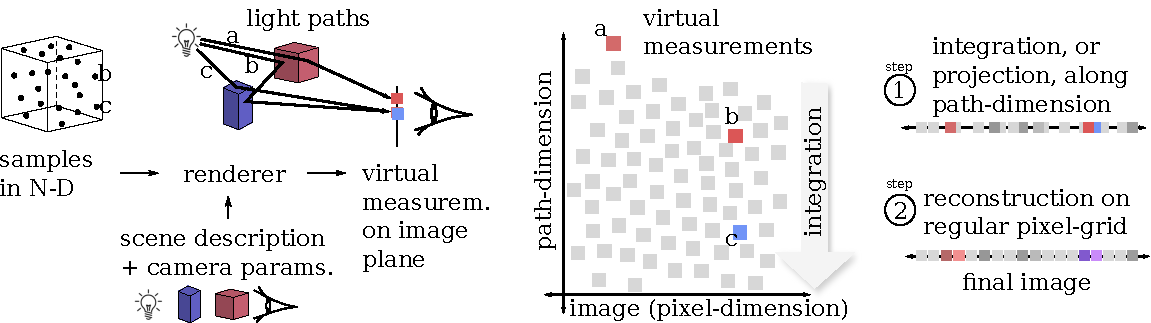
\includegraphics[width=\linewidth]{RenderHL.pdf}
 }
 \caption{\KARTIC{From Subr and Kautz 13. Copyright/license issues?}}
\end{figure}


\section{The interplay between reconstruction and integration}\index{Reconstruction and integration}
Images are typically represented and displayed on a regular grid. Rendering algorithms, however, may estimate virtual measurements at arbitrarily points on the sensor. We refer to the process of resampling the measurements \Ij{}\ on a regular grid as \textit{2D reconstruction}. Some rendering algorithms~\cite{Hachisuka:2008,Egan:2009,Soler:2009} partition the space of paths ($\Omega$ in equation~\ref{eq:measeq}) explicitly into dimensions that are dependent on the camera, such as exposure time and aperture, and those that depend on the scene. Since the sensor is two-dimensional, exposure time is one-dimensional and the aperture is two-dimensional, they estimate virtual measurements in a five-dimensional, camera-dependent space. This involves a reconstruction in 5D followed by a further projection (integration) down to the two-dimensional plane of the sensor. Such a partitioning is exploited for efficient rendering of camera-dependent blur effects resulting from relative motion between the camera and the scene or from defocus due to a finite (rather than infinitesemal) aperture.

\TBC

\section{The role of sampling}
There are two distinctly different applications of sampling in the rendering process. One of them is for reconstruction, either in 2D or in 5D (as described above), and the other is for estimation of integration, which lies at the core of light transport (equation~\ref{eq:measeq}). Most rendering algorithms focus on the latter and perform reconstruction on a two-dimensional regular grid of pixels. Path-tracing, a popular rendering algorithm, proceeds by estimating the virtual image measurement at each pixel by averaging the values of the measurement contributions of a chosen set of paths through each pixel. Each path in the chosen set is obtained via a mapping from a sampling pattern (of appropriate dimensionality) to a set of rays in the scene. These sampling patterns may be stochastic (Monte Carlo sampling) or deterministic patterns that satisfy desirable criteria (Quasi-Monte Carlo). The statistics of the estimates of the virtual measurements yielded by these two broad classes of algorithms are strikingly different, as is the mathematical machinery used for their analyses.  

\TBC

\section{Sources and manifestation of error}\index{Error in rendering}
Error in the context of estimating global illumination~\cite{Arvo94} \GURPRIT{citation missing} arises from three sources: inaccuracies in the  input data or simulation, errors due to discretization and computational errors such as loss of precision. In this course, we focus on the first two sources. The rendered image is represented on a discrete grid, while the distribution of the underlying light energy across the sensor is a continuous function. A major source of error stems from this discretization. Recall that the true continuous function is a high-dimensional integral at each point on the sensor (equation~\ref{eq:measeq}). Any sampling-based approach used to estimate this function results in an approximation whose measured deviation from the true function is known referred to as \textit{approximation error}. Typically approximation error manifests itself in rendered images in one of two perceivably objectionable forms: structured artifacts or as noise. Various metrics, such as L1 norms, L2 norms, PSNR, etc., are used to quantify approximation error.

\TBC 

%----------------------------------------------------------------------------------------
%	CHAPTER 2
%----------------------------------------------------------------------------------------
\chapterimage{ch2.pdf} % Chapter heading image
\chapter{Mathematical preliminaries}
We review relevant mathematical concepts and introduce the notation adopted in this course.


\section{Random variables, expectation and variance}
For the purpose of this course, it will suffice to think of random variates simply as variables whose value is subject to chance. 
 For formal definitions of random variables and functions of random variables, we refer interested readers to introductory textbooks on probability or Monte Carlo simulation~\cite{robertc10}.
 We will restrict ourselves to continuous random variables, denoted using bold capital letters (\RV X, \yii,~etc.), that assume values in some domain \Dom. 
 The relative likelihood for continuous random variables to take on a given value is specified using a (normalized) probability density function (pdf) $\sdsym: \Dom \rightarrow \R$. We denote that \RV X\ is distributed according to \sdn\ by $\RV X \sim \sdn$. The probability that the random variable lies in a subdomain $\Domi{i} \subset \Dom$ is obtained as 
% \begin{equation}
  $\Prob(\RV X \in \Domi{i}) = \DefIntT{\Domi{i}}{}{\sdn}{x}.$
% \end{equation}

A function $\phi:\Dom\rightarrow\R$ evaluated at a location specified by a random variable, $\phi(\RV X)$, is also a random variable.
In this course, we are primarily concerned by the first two moments of random variables (specifically functions of random variables). The first moment, or ``average value'' of a random variable is captured by the mathematical concept of the \textit{expected value} of the random variable. We denote the expected value of \RV X\ as 
$ \Expf{\phi(\RV X)}{\sdsym}   \equiv \DefIntT{\Dom}{}{\phi(x)\;\sdsym(x)}{x}$. 

If the pdf has an expected value, the variance of the random variable is its second central moment which we denote
$\Varf{\phi(\RV X)}{\sdsym} \equiv \Expf{\phi^2(\RV X)}{\sdsym} - \Expf{\phi(\RV X)}{\sdsym}^2$. 
When \RV {X}\ is distributed uniformly within the domain (i.e.~\sdn\ is a constant), we drop the subscript and write the expectation as \Exp{\phi(\RV X)} and the variance as \Var{\phi(\RV X)}.

\TBC 

\section{Estimators}
Consider Monte Carlo estimation of the multidimensional integral $ I = \DefIntT{\Dom}{}{\ifn}{x}, \; \x\in\Dom $.A simple \emph{primary} MC estimator for $I$ is
$\estim{1}\equiv\ifsym(\RV X) , \;\RV X \in \Dom$. When \RV X\ is distributed
uniformly, the estimator is unbiased. That is, its expected value is the integral:$\Exp{\estim{1}}=\Ival$. The function \ifsym(\RV X)\ is itself a random variable with an arbitrary distribution and, typically, a large variance. A more practical MC estimator is obtained by averaging a fixed number of (say \N) primary estimates:  $\estim{\N} = \sum \ifni/\N, \; i=1,2,...,\N$. Such \emph{secondary estimators}  are known to be unbiased and Gaussian-distributed when the primary estimator has finite variance. 

\TBC 

\begin{table}[hbpt]%
\caption{\label{tab:notation}%
Notation used in this course.\TBC}%
\begin{tabular}{rl}%
    \toprule
    Symbol & Definition\\
    \midrule
    \ifn 	&  integrand \\
    $\w(x)$	&  sample weights\\
    \sdn 	&  sampling distribution (pdf) \\
    \estim{\N} 	&  estimate of $I$  using \N\ samples \\
%     \estim{is,\N} 	&  \N-sample importance sampling estimator\\
%     \estim{is,1} 	&  primary (1-sample) imp. samp. estimator\\
    \RV X, \RV Y, \xii, \yii & random variates \\
    $\Exp{\phi(\RV X)}$ 		&
      Expectation: $\DefIntT{\Dom}{}{x\;\phi(x)}{x}$\\[-2pt]
    $\Var{\phi(\RV X)} $ 						&
      Variance : $\DefIntT{\Dom}{}{x\;\phi^2(x)}{x} -
      \DefIntT{\Dom}{}{x\;\phi(x)}{x}$\\
    $\Expf{\phi(\RV X)}{\sdsym} $ &
      Expectation with $ \RV X \sim \sdn$:
$\DefIntT{\Dom}{}{\phi(x)\;\sdsym(x)}{x}$\\[-2pt]
% $\Exp{\phi^2(\RV X)} - \Exp{\phi(\RV X)}^2$\\
    $\Varf{\phi(\RV X)}{\sdsym} $					&
Variance with $ \RV X \sim \sdn$:
  $\DefIntT{\Dom}{}{\phi^2(x)\sdn}{x} -
      (\DefIntT{\Dom}{}{\phi(x)\sdn}{x})^2$\\
\bottomrule
\end{tabular}
\end{table}

\section{The continuous Fourier transform}
\TBC 

\section{Fourier series}
\TBC 

\section{The Discrete Fourier transform}
\TBC 

\section{The Fast Fourier transform}
\TBC 

\section{Power spectral density and the periodogram}
The energy of a signal \ifn\ is generally considered to be the integral of the square of the signal (over its entire domain). Due to Parseval's theorem, this may also be expressed as the integral of the square of the Fourier spectrum of the signal over all frequencies. The integrand in this expression of power, $|\IFn|^2$, is referred to as the \textit{power spectrum} of \ifn. For discrete signals, the corresponding spectral density is called a \emph{periodogram}. We denote the periodogram of a discretised function $S(x)$ as $\PowerSpec{S}(\fv)$, which represents the squared amplitude of the Fourier coefficients corresponding to each frequency. 

\TBC
%----------------------------------------------------------------------------------------
%	CHAPTER 3
%----------------------------------------------------------------------------------------
\chapterimage{ch3.pdf} % Chapter heading image
\chapter{Sampling for reconstruction}
The reconstruction problem entails approximating a function $\ifsym:\Dom\rightarrow\R$ as $\appr{\ifsym}(x_i), \; x_i\in\Dom, \;i=1,2,3,...,M$ given $\ifsym(y_i), \; y_i \in \Dom, \;j=1,2,3,...,\N$, where the sets of points $\{x_i\}$ and $\{y_j\}$ are mutually exclusive. If $\appr{\ifsym}(y_j) = \ifsym(y_j),\;\forall j$, the process is referred to as interpolation. This problem has received much attention in the signal processing literature~\cite[chapters~5~\&~6]{engineering2008handbook} as well as in the rendering community~\cite{Wold85,Cook:1986:SSC,mitchell87a}. Such analyses have yielded effective reconstruction filters that are used in modern renderers, especially in low-dimensional domains such as the image plane.

Reconstruction is akin to nonlinear regression~\cite{GVK394929411}, a popular problem in the statistics (and more recently machine learning) literature, which offers effective solutions in high-dimensional settings when the approximand exhibits stationarity or accurate solutions for smooth and low-dimensional approximands. In rendering, the underlying functions represent a multitude of combinations (products, convolutions and sums) of a variety of non-stationary processes such as spatio-directional lighting, hard shadows, sharp reflections, textured materials, etc. The resulting discontinuities and variations in the radiant light energy (radiance function) across space-angle-time pose immense challenges which state of the art methods in non-linear regression are unable to cope with.

The reconstruction process generally consists of two steps. First, for any point $x$ in the domain, the influence of each of the $\ifsym(y_j)$ samples is specified using some \textit{weighting kernel} on the distance between $x$ and $y_i$ (typically Euclidean). Then, at each of the $x_i$, the approximate value is obtained by summing up the distance-weighted contributions of each of the $\ifsym(y_j)$. Depending on the choice of the kernel and the strategy for determining weights, the resulting methods are known by different names: Kernel Smoothers, Radial Basis Functions, Shepherd's method, etc.  

\section{Aliasing in reconstruction}
The general reconstruction process (above) may be written in terms of the underlying function (or signal). The samples, $\ifsym(y_i), \; y_i \in \Dom$, can be represented as the  product of the true (often unknown) function \ifn\ with a sampling function of the form $S(x) = \sum\limits_{j=1}^{\N} \updelta(x-y_j)$. 
If $K(r)$ represents the kernel weight at a distance of $r$, the continuous approximand and its Fourier dual are
\begin{equation} \label{eq:recons}
 \appr{\ifsym}(x) = \left(\ifn . S(x) \right) \conv K(x) \Fdual 
 \appr{\IFsym}(\fv) = \left(\IFn \conv \FTsym{S}(\fv)\right) . \FTsym{K}(\fv) 
\end{equation}
where \conv\ denotes convolution. That is, the effect of sampling can be seen in the Fourier domain as one of generating spurious replicas of \IFsym\, created due to the convolution with $\FTsym{S}$, which potentially hinders perfect reconstruction.   The kernel, on the other hand, can be viewed as a low-pass filter which suppresses replicated, or aliased, copies of the true function's spectrum at high frequencies. 

If \ifn\ contains frequencies less than $\fv_b$ (is band-limited), if the sampling spectrum does not contain frequencies lower than $2\fv_b$, and if the kernel is a low-pass filter suppressing frequencies above $\fv_b$, the resulting reconstruction will be perfect. If these conditions are not satisfied, the approximation will contain error. The first potential source of error is that \ifn\ is not bandlimited and hence, regardless of the sampling function, the low-pass effect of the kernel results in the loss of high-frequencies. The other main source of error is due to the sampling spectrum containing low frequencies, which results in a \FTsym{\appr{\ifsym}}\ that contains a superposition of \IFn\ with its aliased copies.

\section{Antialiasing}
The error introduced by aliasing either appears as coherent structure or as noise, depending on the choice of sampling spectrum. Sampling on a regular grid corresponds to multiplication with a Dirac-train or Shah function, whose Fourier spectrum remains a Shah function. If the samples are not sufficiently dense in the image plane, the resulting spectrum contains impulses at lower frequencies which cause aliasing in the form of regular structure that has been shown to be particularly unpleasant to our perceptual system. If the function being reconstructed is bandlimited, and in the absence of a sampling budget, the sampling rate may be increased to eliminate aliasing. However, if the function contains arbitrarily high frequencies, a simple strategy is to introduce randomness in the spectrum thereby transforming coherent artifacts into visual noise. This has shown to be less objectionable to our visual systems.

\TBC

\section{Halftoning}
Halftoning is the process of determining a sampling function $S(x)$ so that a kernel density estimate of the sampled function $\appr{\ifsym}(x) = \ifn.S(x)$ provides the best approximation to \ifn. It is a special case of reconstruction where the kernel is implicit and dependent on our visual systems. Halftoning methods strive to identify sampling functions for which the \textit{perceived} sampled function is as close to \ifn\ as possible. This may be achieved by varying the distributions of the samples, by weighting them or using a combination of both. Densely sampled regions of the sampled function are perceived to have darker tone. 

\TBC

\section{Antialiasing as integration}
Antialiasing is commonly viewed as an integration problem. The value to be assigned to a pixel is often estimated by averaging sampled values within a square around the pixel. That is, pixels are viewed as little squares and the values assigned to pixels are obtained by integrating the underlying function within their respective squares. On the contrary, if pixels are viewed as simply being points on the image plane~\cite{smith1995pixel}, this choice of integrating within the pixel appears to be an arbitrary choice. That is, it corresponds to performing reconstruction on the image plane exactly as in equation~\ref{eq:recons}, with $K(x)$ chosen to be a box with a width that is half the inter-pixel distance, followed by resampling of $\appr{\ifsym}(x)$ on a regular grid. Although this view of antialiasing is better than not performing antialiasing, it is well known that the box-filter is not the ideal choice. Modern renderers offer a variety of choices for the pixel reconstruction filter, since its choice is dependent on the rendering algorithm chosen and the corresponding sampling patterns used for estimating light energy arriving at the pixel~\cite[section~7.6]{Pharr:2010:PBR:1854996}.

\TBC
%----------------------------------------------------------------------------------------
%	CHAPTER 4
%----------------------------------------------------------------------------------------
\chapterimage{ch4.pdf} % Chapter heading image
\chapter{Estimating integrals}
The goal of rendering is to estimate the quantity of radiant light energy impinging on the various pixels (or cells) distributed on a virtual observer's camera (or eye). Current renderers perform this via physically-based simulation of light, following its intricate combinations of reflections within the scene. The virtual measurement \Ij {\xs} at a point \xs\  on the sensor~\cite{VeachChapter8} is
\begin{eqnarray} \label{eq:measeq}
 \Ij {\xs} & = & \DefInt{\Omega}{}{f_\xs(\pth)}{\mu(\pth)}
\end{eqnarray}
where the measurement contribution function, $f_\xs(\pth)$, is the importance-weighted radiance arriving at \xs\ along the path \pth\ and $\mu(\pth)$ is a measure on the space of all paths $\Omega$. The paths \pth\ span space as well as time and may be of arbitrarily high dimensionality. Thus, physically-based rendering requires the esimation of high-dimensional integrals at each point \xs\ on the virtual sensor. 

The exact nature of the integrand depends on the complexity and structure of the scene being rendered, along with detailed modelling of the constituent materials and shapes.  In general, the integrand is high-dimensional, discontinuous and costly to evaluate. Each evaluation of the integrand requires many rays to be traced within the environment, along with estimation of the radiant light energy along that path formed by linking the rays together. 
The rendering community strives to estimate such integrals with low error as well as low computational cost.


\section{Numerical integration via sampling}
Henceforth in this chapter, we abstract away the details about the integrand and domain of integration (equation~\ref{eq:measeq}) that is encountered in rendering. We study the integration problem in the canonical domain.  
Our goal is to analyze the of quality of numerical integration, within the interval $[0,\Tx]$, of a function $\ifsym: \R \mapsto \R^{+}$. 
% in terms of the Fourier spectrum of the underlying sampling strategy. 
For example, a \textit{primary} Monte Carlo estimator $\estim{1} = \ifsym(\xii)$ for the integral
\begin{equation} \label{eq:integcanonical}
I \equiv \frac 1 \Tx \DefInt{0}{\Tx}{\ifn }{\x}  
\end{equation}
is well known to be unbiased if the  single sample $\xii \in [0,\Tx] $ is drawn from a constant probability distribution function (pdf) within the domain $[0,\Tx]$.~i.e.~$\Exp{\estim{1}} = I$.
The corresponding secondary estimator, obtained by averaging \N\ primary estimates at different \xii\ has the same expected value. However, the averaging scales the variance down by a factor of $\N$.~i.e.~$\Var{\estim{\N}} = \Var{\estim{1}}/\N.$ 

\TBC
\begin{figure}
 \centering
 {
  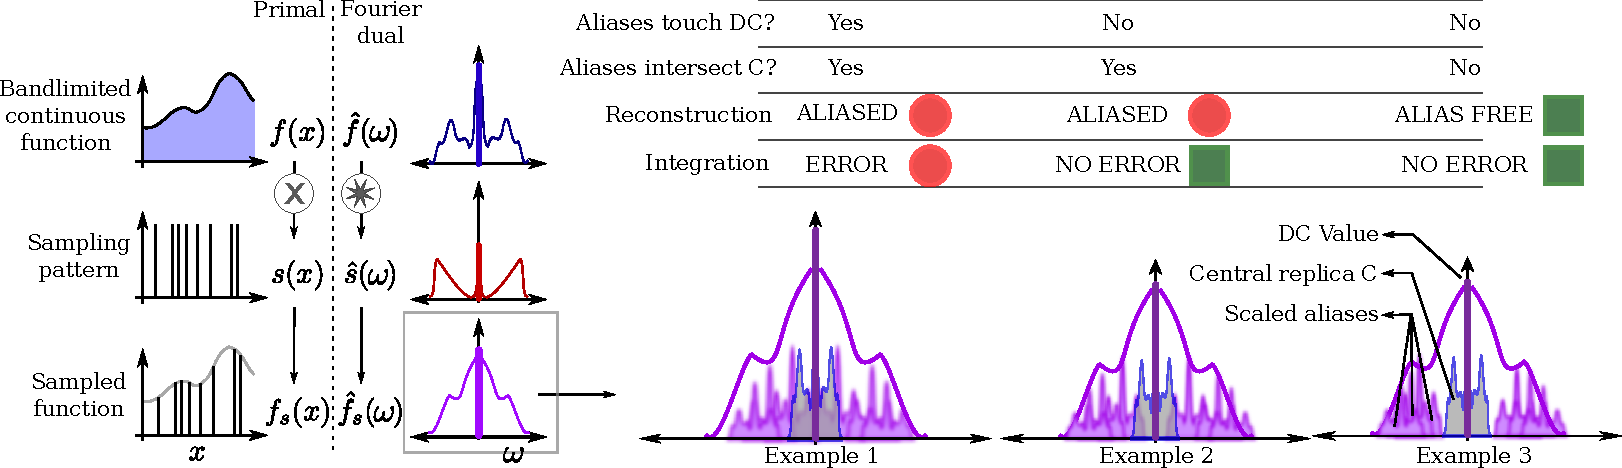
\includegraphics[width=\linewidth]{IntegRecons.pdf}
 }
 \caption{\KARTIC{From Subr and Kautz 13. Copyright/license issues?}}
\end{figure}

\section{Error due to sampling}
\subsection{Bias}
\TBC
\subsection{Consistency}
\TBC
\subsection{Variance (uncertainty of estimates)} 
\GURPRIT{
Unless I am missing something I don't see why uncertainty refers to Variance. For me uncertainty is a relative concept. For example, 
the variance of a kernel in the primal and the fourier domain cannot be predicted simultaneously at a given frequency. Reducing variance in one domain would increase variance in the other, which is what 
uncertainty is all about. }
\KARTIC{Random variables introduce uncertainty. Variance is one form of the quantification of uncertainty. If you are estimating Variance, then you can talk about uncertainty of the variance estimates. I like to pose the process of quantifying error in the estimates as a form of uncertainty propagation (\url{https://en.wikipedia.org/wiki/Propagation_of_uncertainty}). That is, if we know the uncertainty in the sampling patterns, can we estimate uncertainty in the final estimates?}

\TBC
\subsection{Convergence}
\TBC
\subsection{Homogenization}
\TBC

\section{Monte Carlo integration in the Fourier domain}
Monte Carlo sampling can be represented as an inner product of the integrand \ifn\ and the sampling pattern \sfn\ which is composed of a sum of impulses (delta functions) normalized by the number of impulses \GURPRIT{maybe we can also mathematically write \sfn\ }. Since inner products are preserved under Fourier Transforms, the na\"ive estimator 
\begin{equation}
  \estim{\N} \quad = \quad \DefInt{\Dom}{}{\ifn \sfn}{x} \quad = \quad 
  \DefInt{\Omega}{}{\SF \; \IFsym^*(\fv) }{\fv}.
\end{equation}

\TBC 

%\section{Assessing sampling patterns based on their spectra}
%
%!TEX root = main.tex
%
% Start with sampling patterns 
%
%
\section{Assessing sampling patterns based on their spectra}

\subsection{Qualitative assessment using periodograms}
Following the seminal work by Robert Ulichney on \emph{blue noise} dithering~\cite{Ulichney:87:halftoning}, sampling patterns with minimal energy in the low frequency zone of their power spectra are believed to be preferable, for applications such as stippling and numerical integration. Tools such as the \emph{periodogram} and its radially-averaged profile were introduced to the graphics community about three decades ago, and were primarily used for qualitative comparisons of sampling patterns. 
% Ulichney also proposed to use \emph{radially-averaged} power spectra, as a means of explicitly visualizing 
% which can be mathematically written as:
% %
% \begin{align}
% \RadialPowerSpec{\Sampling}(\RadialFreq) = \int_{\FreqVar = \RadialFreq} \PowerSpec{\Sampling}(\FreqVar) \Diff \FreqVar \,.
% \end{align}
%
%Periodograms does help in investigating low frequency zone region of sampling power spectra but it is not always possible to get a precise behaviour of periodograms for various sampling patterns like jitter and Poisson Disk. This is where radially averaged power spectra comes handy. By performing radial averaging of sampling power spectra we can get a closer and better look at the low frequency as well as the mid to high frequency regions of the sampling power spectra.
These tools have been used to compare the qualities of blue noise sampling patterns generated using various algorithms, and have been extended for comparisons between spatially-varying sampling distributions~\cite{Wei:2011:DDA}. 

\subsection{Quantifying error using the statistics of sampling spectra}
More recently, the focus has been on quantification of estimation error in the Fourier domain. That is, the error of an estimator (e.g.~\estim{1} for $I$ in equation~{eq:integcanonical}) has been expressed in terms of the Fourier spectra of the integrand and sampling function. 
% Monte Carlo integration has been only recently unfolded in a step by step manner starting from Durand~\cite{durand2011frequency}, Subr and Kautz~\cite{Subr:2013:FAS}, and then by 
% shortcite
Durand~\cite{durand2011frequency} derived mean-squared error (MSE) as the inner product of the spectral densities of the integrand and sampling function, 
\begin{equation} \label{eq:durand11}
   \Exp{(I-\estim{1})^2} = \DefInt{\Omega}{}{|\IFn|^2 \; \Exp{|\SF|^2}}{\fv},
\end{equation}
and verified that the convergence rate of the MSE of \estim{\N}\ is indeed $1/\N$. Following this work, it was shown~\cite{Subr:2013:FAS} that the bias and variance of \estim{1}\ may be expressed separately in terms of the spectra. They derived
\begin{eqnarray}
  \Exp{I-\estim{1}} &=& I - \DefInt{\Omega}{}{\Exp{\SF} \; \IFn }{\fv}, \quad \mathrm{and} \\
    \Var{\estim{1}} &\leq& \DefInt{\Omega}{}{\Var{\SF} \; |\IFn|^2}{\fv}
\end{eqnarray}
as the expressions for bias and variance respectively.~i.e.~An estimator's bias is dependant on the relationship between the expected Fourier spectrum of the sampling pattern and the integrand's spectrum. The second equation, shows that the estimator's variance is bounded by the variance present in the sampling spectrum relative to the spectral density of the integrand. Subsequently, these results were collated and the expression for the variance was reformulated~\cite{Pilleboue:2015:VAM} for homogenized (unbiased) Monte Carlo estimators as
%
\begin{equation} \label{eq:pillebouevar}
\Var{\estim{1}} 
= \DefInt{\Omega}{}{\Exp{|\SF|^2}\;|\IFn|^2}{\fv} 
= \DefInt{\Omega}{} {\Exp{\PowerSpec{\SFsym}(\fv)} \PowerSpec{\ifsym}(\fv)} {\fv} 
\end{equation}
which is identical to Durand's derivation of MSE (equation~\ref{eq:durand11}) for a general (possibly biased) \GURPRIT{I think Durand derived the variance for only random (white noise) samples, as he mentioned. Pilleboue obtained the same variance formulation but it was generalised to all samplers, thanks to the homogenization property} estimator. However, the homogenized perspective yields important insights and results on the convergence rate of estimators. \GURPRIT{I don't understand this statement, are you saying thanks to homogenization the convergence rates can be obtained ? }
%

\subsection{Quantifying convergence using periodograms}
The primary advantage of studying the variance of the homogenized (equation~\ref{eq:pillebouevar}) estimator was that it allowed an analysis of the convergence rate of estimators in terms of their power spectra. In addition, the homogenization process provides an elegant means of quantitatively comparing errors due to random (Monte Carlo) sampling patterns with deterministic (quasi Monte Carlo) patterns. 
\GURPRIT{We should be careful while making statements about the QMC methods. Although we can use the homogenization property for any sampling pattern we do not give any insights on how our Fourier analysis would yield convergence rates for QMC methods. This is tricky because QMC methods like Sobol can give different power spectra depending on the number of samples used. Pilleboue et al's method 
do not handle these cases.
}
\TBC
%
\section{Analysis beyond the canonical domain}
\TBC
\subsection{Spherical domain}
\TBC
\subsection{General domains}
\TBC
\subsection{Gradient domain}
\TBC
\section{Manifestation of error in rendering}
\TBC

%----------------------------------------------------------------------------------------
%	CHAPTER 5
%----------------------------------------------------------------------------------------
\chapterimage{ch5.pdf} % Chapter heading image
\chapter{Popular sampling patterns} \label{ch:samplingpatterns}
In this chapter, we describe sampling strategies that are popularly used in modern renderers. For each of these, we provide insight on its error, explain the contexts where its behaviour is best and/or worst and also comment on its expected convergence rate using its homogenized periodogram.

\TBC

\section{Classical}
\subsection{Random sampling}
\TBC
\subsection{Jittered sampling}
\TBC
\subsection{Uniform jittered sampling}
\TBC

\section{Quasi-Monte Carlo}
\subsection{Sobol sequence}
\TBC
\subsection{Hammersley sequence}
\TBC
\subsection{Latin hypercube sampling}
\TBC

\section{Blue noise}
\GURPRIT{
I think the we can cover different classes of samplers if we can simply rename the subsections of this 
section to the following: \\
- Dart throwing based methods \\
- Relaxation based methods \\
- Tiling based methods 
}
\KARTIC{I've modified CCVT to Relaxation-based. However, I think Poisson-disk sampling is the general idea for which dart-based methods are used (rather than the other way around), so I've kept the first subsection PDisk}

\GURPRIT{This is correct but we can also generate Poisson disk sampling using relaxation based methods 
and/or tile based methods (Kopf et al.2006, Lagae and Dutre 2008). I was actually proposing to separate the generation process of sampling patterns. Dart throwing is one way of generating samples, which by 
default give Poisson disk patterns. 
}
\subsection{Poisson-disk sampling}
\TBC
\subsection{Relaxation-based methods}
\TBC
\subsection{Tiling-based methods}
\TBC

\section{Synthesis of sampling patterns with targeted spectral profiles}
\TBC

%----------------------------------------------------------------------------------------
%	CHAPTER 6
%----------------------------------------------------------------------------------------
\chapterimage{ch6.pdf} % Chapter heading image
\chapter{Case studies}
In this chapter, we invent a suite of tests that may be used to compare the efficacy of sampling patterns when used in numerical integration. We will then tabulate this comparison, identifying the strengths and weaknesses of the different sampling strategies described in chapter~\ref{ch:samplingpatterns}. Our test suite will encompass a variety of integrands of various dimensionalities as well as smoothness criteria. We will make our code available to facilitate the comparison of any sampling patterns that may be proposed in the future with methods in our chosen set of algorithms. 

\section{1D integrands}
\TBC 

\subsection{Smooth functions}
\TBC 
\subsection{Functions with discontinuities}
\TBC 
\section{2D integrands}
\TBC 
\subsection{Smooth functions}
\TBC 
\subsection{Functions with discontinuities}
\TBC 
\subsection{Sub-pixel integration}
\TBC 
\section{Rendering test suite}
\TBC 

% 
% \section{Figure}\index{Figure}
% 
% \begin{figure}[h]
% \centering
\includegraphics[scale=0.5]{placeholder}
% \caption{Figure caption}
% \end{figure}

%----------------------------------------------------------------------------------------
%	BIBLIOGRAPHY
%----------------------------------------------------------------------------------------
\chapterimage{biblio.pdf} % Chapter heading image

% \chapter*{Bibliography}
% \nocite{*}
% \section*{Books}
% \addcontentsline{toc}{section}{Books}
% \printbibliography[heading=bibempty,type=book]
% \section*{Articles}
% \addcontentsline{toc}{section}{Articles}
% \printbibliography[heading=bibempty]
\bibliographystyle{unsrt}
\bibliography{bibliography.bib}
\addcontentsline{toc}{chapter}{\textcolor{ocre}{Bibliography}}

%----------------------------------------------------------------------------------------
%	INDEX
%----------------------------------------------------------------------------------------

\cleardoublepage
\phantomsection
\setlength{\columnsep}{0.75cm}
\addcontentsline{toc}{chapter}{\textcolor{ocre}{Index}}
\printindex

%----------------------------------------------------------------------------------------

\end{document}